\documentclass[pstricks,border=12pt]{amsart}
\usepackage{pgfplots}
\begin{document}
In this informal article I will explain popularly my concept of generalized limit of arbitrary (discontinuous) function.

Consider some function~$f$:

\begin{figure}[ht]
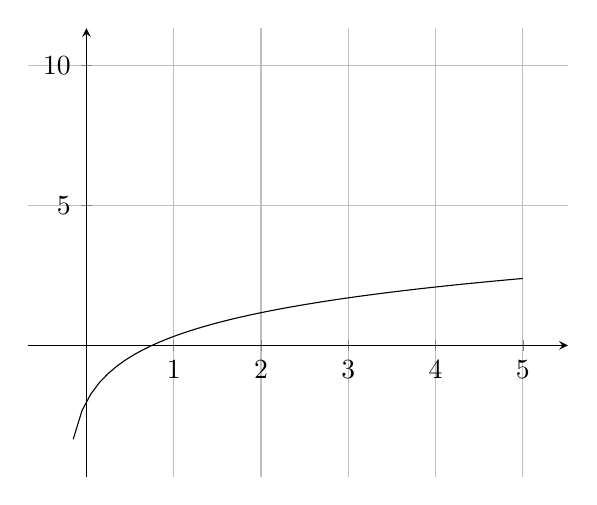
\begin{tikzpicture}
\begin{axis}[grid=both,
          xmax=5,ymax=10,
          axis lines=middle,
          restrict y to domain=-7:7,
          enlargelimits]
\addplot[domain=-5:5,samples=100]  {log2(x+.25)};
\end{axis}
\end{tikzpicture}
\end{figure}

Take it's infinitely small fragment (in our example, an infinitely small interval for~$x$ around zero; see the actual book for an explanation what is infinitely small):

\begin{figure}[ht]
\begin{tikzpicture}
\begin{axis}[grid=both,
          xmax=5,ymax=10,
          axis lines=middle,
          restrict y to domain=-7:7,
          enlargelimits]
\addplot[domain=-0.1:0.1,samples=100]  {log2(x+.25)};
\end{axis}
\end{tikzpicture}
\end{figure}
\end{document}
